%50 minutos -> 40 slides no máximo
\documentclass[
    mode=present,
    style=dvn,
    paper=screen,
    display=slidesnotes,
    size=14pt,
]{powerdot}

\usepackage[utf8]{inputenc}
\usepackage[sfdefault]{universalis}
\usepackage[T1]{fontenc}
\usepackage[brazilian]{babel}
\usepackage{amsmath,amsthm,amssymb,amsfonts,mathtools}
\usepackage{tcolorbox}
%\usepackage{enumerate}

\newcommand*\plus{+{}}
\newcommand*\boxSizeOfMax[1]{\makebox[\widthof{Max}][c]{#1}}
\newcommand{\N}{\mathbb{N}}
\newcommand{\Z}{\mathbb{Z}}
%\renewcommand{\O}[1]{$\mathcal{O}(#1)$}
\theoremstyle{plain}
\newtheorem{thm}{Teorema}
\newtheorem{lem}[thm]{Lema}
\newtheorem{prop}[thm]{Proposição}
\newtheorem*{cor}{Corolário}

\theoremstyle{definition}
\newtheorem{defn}{Definição}
\newtheorem{conj}{Conjectura}
\newtheorem{exmp}{Exemplo}

\theoremstyle{remark}
\newtheorem*{rem}{Observação}

\pdsetup{
     %lf=Minimização d,
     counters={thm,defn,conj,exmp},
     %rf=~\arabic{},
     palette=navy,
     trans=Wipe,
     theslide=~\arabic{slide},
     list={itemsep=6pt}
 }

\tcbset{colback=pdcolor4,colframe=pdcolor1,coltext=pdcolor1}

\title{Teoria da Complexidade \\
    \small Notação Assintótica\\}
\author{\smallskip Prof. Diego Noble \\%
\texttt{\href{mailto:diegovnoble@gmail.com}{\color{pdcolor4}diegovnoble@gmail.com}}}%
%\texttt{\href{http://www.inf.ufrgs.br/~dvnoble/}{\color{pdcolor4}http://www.inf.ufrgs.br/{\raise.17ex\hbox{$\scriptstyle\sim$}}dvnoble/}}}
\date{\today}

\begin{document}

\maketitle

\begin{slide}{Introdução}
    \vspace{\stretch{1}}
    \begin{itemize}
        \item Analisar algoritmos significa determinar os recursos computacionais que
        o algoritmo requer conforme o tamanho da entrada aumenta.
    \end{itemize}
    \bigskip
    
    $\rightarrow$ O objetivo desta aula é ``concretizar'' esta ideia de análise.\pause

    $\rightarrow$ Esse é passo inicial para compreender o conceito de \textit{tratabilidade}.
    \vspace{\stretch{1}}
\end{slide}

% \begin{slide}{Pior caso}
%     \vspace{\stretch{1}}
%     \begin{itemize}
%         \item 
%     \end{itemize}
%     \vspace{\stretch{1}}
% \end{slide}

\begin{slide}{Conteúdo}
    \vspace{\stretch{1}}
    \Large
    \tableofcontents[content=sections]
    \vspace{\stretch{1}}
\end{slide}
\section{Conceito de Eficiência}
\begin{slide}{Complexidade}
    \vspace{\stretch{1}}
    \Large
    \begin{itemize}
    \item \myemph{Encontrar algoritmos eficientes para solucionar problemas computacionais.}
    \end{itemize}
    Mas o que é ``\myemph{executar rapidamente}''?
    \vspace{\stretch{1}}
\end{slide}

\begin{slide}{Eficiência I}
    \vspace{\stretch{1}}
    \Large
    \begin{defn}
        Um algoritmo é eficiente se, quando implementado, executa rapidamente para instâncias reais como entrada.
    \end{defn}
    \vspace{\stretch{1}}
\end{slide}

\begin{slide}{Eficiência II}
    \vspace{\stretch{1}}
    \Large
    \begin{defn}
        Um algoritmo é eficiente se, qualitativamente e em seu pior caso, tem um desempenho superior a um algoritmo de força-bruta.
    \end{defn}
    \vspace{\stretch{1}}
\end{slide}

\begin{slide}{Eficiência III}
    \vspace{\stretch{1}}
    \Large
    \begin{defn}
        Um algoritmo é eficiente se o seu tempo de execução é polinomial.\pause
    \end{defn}
    \myemph{Mas $n^{100}$ é melhor que $n^{1+0.02(\log n)}$?}
    \vspace{\stretch{1}}
\end{slide}

\section{Notação Assintótica}

\begin{slide}{\textit{Big-oh} $\mathcal{O}$}
    \vspace{\stretch{1}}
    \begin{defn}
        \myemph{Limite assintótico superior} $T(n)$ é $O(f(n))$ \textit{se} existem constantes $c>0$ e $n_0 \geq 0$ tal que $\forall n \geq n_0$, é o caso que \myemph{$T(n) \leq c.f(n)$}.\pause
    \end{defn}
    Dizemos neste caso que $T(n)$ é limitada superiormente por $f(n)$.
    \bigskip
    \begin{tcolorbox}[title=Exemplo]
        $T(n) = 10n + 8, f(n)=n^2, c = 5, n_0 = 2$ 
    \end{tcolorbox}
    \vspace{\stretch{1}}
\end{slide}

\begin{slide}{\textit{Big-oh} $\mathcal{O}$}
    \vspace{\stretch{1}}

    \begin{figure}
        % GNUPLOT: LaTeX picture with Postscript
\begingroup
  \makeatletter
  \providecommand\color[2][]{%
    \GenericError{(gnuplot) \space\space\space\@spaces}{%
      Package color not loaded in conjunction with
      terminal option `colourtext'%
    }{See the gnuplot documentation for explanation.%
    }{Either use 'blacktext' in gnuplot or load the package
      color.sty in LaTeX.}%
    \renewcommand\color[2][]{}%
  }%
  \providecommand\includegraphics[2][]{%
    \GenericError{(gnuplot) \space\space\space\@spaces}{%
      Package graphicx or graphics not loaded%
    }{See the gnuplot documentation for explanation.%
    }{The gnuplot epslatex terminal needs graphicx.sty or graphics.sty.}%
    \renewcommand\includegraphics[2][]{}%
  }%
  \providecommand\rotatebox[2]{#2}%
  \@ifundefined{ifGPcolor}{%
    \newif\ifGPcolor
    \GPcolortrue
  }{}%
  \@ifundefined{ifGPblacktext}{%
    \newif\ifGPblacktext
    \GPblacktextfalse
  }{}%
  % define a \g@addto@macro without @ in the name:
  \let\gplgaddtomacro\g@addto@macro
  % define empty templates for all commands taking text:
  \gdef\gplbacktext{}%
  \gdef\gplfronttext{}%
  \makeatother
  \ifGPblacktext
    % no textcolor at all
    \def\colorrgb#1{}%
    \def\colorgray#1{}%
  \else
    % gray or color?
    \ifGPcolor
      \def\colorrgb#1{\color[rgb]{#1}}%
      \def\colorgray#1{\color[gray]{#1}}%
      \expandafter\def\csname LTw\endcsname{\color{white}}%
      \expandafter\def\csname LTb\endcsname{\color{black}}%
      \expandafter\def\csname LTa\endcsname{\color{black}}%
      \expandafter\def\csname LT0\endcsname{\color[rgb]{1,0,0}}%
      \expandafter\def\csname LT1\endcsname{\color[rgb]{0,1,0}}%
      \expandafter\def\csname LT2\endcsname{\color[rgb]{0,0,1}}%
      \expandafter\def\csname LT3\endcsname{\color[rgb]{1,0,1}}%
      \expandafter\def\csname LT4\endcsname{\color[rgb]{0,1,1}}%
      \expandafter\def\csname LT5\endcsname{\color[rgb]{1,1,0}}%
      \expandafter\def\csname LT6\endcsname{\color[rgb]{0,0,0}}%
      \expandafter\def\csname LT7\endcsname{\color[rgb]{1,0.3,0}}%
      \expandafter\def\csname LT8\endcsname{\color[rgb]{0.5,0.5,0.5}}%
    \else
      % gray
      \def\colorrgb#1{\color{black}}%
      \def\colorgray#1{\color[gray]{#1}}%
      \expandafter\def\csname LTw\endcsname{\color{white}}%
      \expandafter\def\csname LTb\endcsname{\color{black}}%
      \expandafter\def\csname LTa\endcsname{\color{black}}%
      \expandafter\def\csname LT0\endcsname{\color{black}}%
      \expandafter\def\csname LT1\endcsname{\color{black}}%
      \expandafter\def\csname LT2\endcsname{\color{black}}%
      \expandafter\def\csname LT3\endcsname{\color{black}}%
      \expandafter\def\csname LT4\endcsname{\color{black}}%
      \expandafter\def\csname LT5\endcsname{\color{black}}%
      \expandafter\def\csname LT6\endcsname{\color{black}}%
      \expandafter\def\csname LT7\endcsname{\color{black}}%
      \expandafter\def\csname LT8\endcsname{\color{black}}%
    \fi
  \fi
    \setlength{\unitlength}{0.0500bp}%
    \ifx\gptboxheight\undefined%
      \newlength{\gptboxheight}%
      \newlength{\gptboxwidth}%
      \newsavebox{\gptboxtext}%
    \fi%
    \setlength{\fboxrule}{0.5pt}%
    \setlength{\fboxsep}{1pt}%
\begin{picture}(5040.00,3772.00)%
    \gplgaddtomacro\gplbacktext{%
      \colorrgb{0.12,0.21,0.34}%
      \put(3369,1627){\makebox(0,0)[l]{\strut{}$T(n)$}}%
      \colorrgb{0.90,0.29,0.27}%
      \put(2944,3194){\makebox(0,0)[l]{\strut{}$c.f(n)$}}%
    }%
    \gplgaddtomacro\gplfronttext{%
      \csname LTb\endcsname%
      \put(176,1940){\rotatebox{-270}{\makebox(0,0){\strut{}$tempo$}}}%
      \put(2519,154){\makebox(0,0){\strut{}$n$}}%
    }%
    \gplbacktext
    \put(0,0){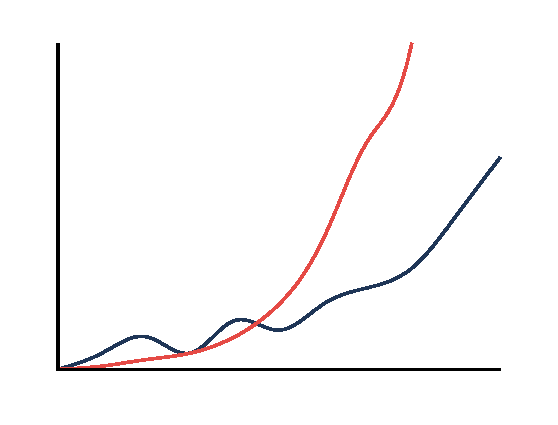
\includegraphics{big}}%
    \gplfronttext
  \end{picture}%
\endgroup

        \caption{$T(n){\in}\mathcal{O}(f(n))$}
    \end{figure}
    \vspace{\stretch{1}}
\end{slide}

\begin{slide}{$\Omega$}
    \vspace{\stretch{1}}
    \begin{defn}
        \myemph{Limite assintótico inferior} $T(n)$ é $\Omega(f(n))$ \textit{se} existem constantes $c>0$ e $n_0 \geq 0$ tal que $\forall n \geq n_0$, é o caso que \myemph{$T(n) \geq c.f(n)$}.\pause
    \end{defn}
    Dizemos neste caso que $T(n)$ é limitada inferiormente por $f(n)$.
    \bigskip
\vspace{\stretch{1}}
\end{slide}

\begin{slide}{$\Omega$}
    \vspace{\stretch{1}}
    \begin{figure}
        % GNUPLOT: LaTeX picture with Postscript
\begingroup
  \makeatletter
  \providecommand\color[2][]{%
    \GenericError{(gnuplot) \space\space\space\@spaces}{%
      Package color not loaded in conjunction with
      terminal option `colourtext'%
    }{See the gnuplot documentation for explanation.%
    }{Either use 'blacktext' in gnuplot or load the package
      color.sty in LaTeX.}%
    \renewcommand\color[2][]{}%
  }%
  \providecommand\includegraphics[2][]{%
    \GenericError{(gnuplot) \space\space\space\@spaces}{%
      Package graphicx or graphics not loaded%
    }{See the gnuplot documentation for explanation.%
    }{The gnuplot epslatex terminal needs graphicx.sty or graphics.sty.}%
    \renewcommand\includegraphics[2][]{}%
  }%
  \providecommand\rotatebox[2]{#2}%
  \@ifundefined{ifGPcolor}{%
    \newif\ifGPcolor
    \GPcolortrue
  }{}%
  \@ifundefined{ifGPblacktext}{%
    \newif\ifGPblacktext
    \GPblacktextfalse
  }{}%
  % define a \g@addto@macro without @ in the name:
  \let\gplgaddtomacro\g@addto@macro
  % define empty templates for all commands taking text:
  \gdef\gplbacktext{}%
  \gdef\gplfronttext{}%
  \makeatother
  \ifGPblacktext
    % no textcolor at all
    \def\colorrgb#1{}%
    \def\colorgray#1{}%
  \else
    % gray or color?
    \ifGPcolor
      \def\colorrgb#1{\color[rgb]{#1}}%
      \def\colorgray#1{\color[gray]{#1}}%
      \expandafter\def\csname LTw\endcsname{\color{white}}%
      \expandafter\def\csname LTb\endcsname{\color{black}}%
      \expandafter\def\csname LTa\endcsname{\color{black}}%
      \expandafter\def\csname LT0\endcsname{\color[rgb]{1,0,0}}%
      \expandafter\def\csname LT1\endcsname{\color[rgb]{0,1,0}}%
      \expandafter\def\csname LT2\endcsname{\color[rgb]{0,0,1}}%
      \expandafter\def\csname LT3\endcsname{\color[rgb]{1,0,1}}%
      \expandafter\def\csname LT4\endcsname{\color[rgb]{0,1,1}}%
      \expandafter\def\csname LT5\endcsname{\color[rgb]{1,1,0}}%
      \expandafter\def\csname LT6\endcsname{\color[rgb]{0,0,0}}%
      \expandafter\def\csname LT7\endcsname{\color[rgb]{1,0.3,0}}%
      \expandafter\def\csname LT8\endcsname{\color[rgb]{0.5,0.5,0.5}}%
    \else
      % gray
      \def\colorrgb#1{\color{black}}%
      \def\colorgray#1{\color[gray]{#1}}%
      \expandafter\def\csname LTw\endcsname{\color{white}}%
      \expandafter\def\csname LTb\endcsname{\color{black}}%
      \expandafter\def\csname LTa\endcsname{\color{black}}%
      \expandafter\def\csname LT0\endcsname{\color{black}}%
      \expandafter\def\csname LT1\endcsname{\color{black}}%
      \expandafter\def\csname LT2\endcsname{\color{black}}%
      \expandafter\def\csname LT3\endcsname{\color{black}}%
      \expandafter\def\csname LT4\endcsname{\color{black}}%
      \expandafter\def\csname LT5\endcsname{\color{black}}%
      \expandafter\def\csname LT6\endcsname{\color{black}}%
      \expandafter\def\csname LT7\endcsname{\color{black}}%
      \expandafter\def\csname LT8\endcsname{\color{black}}%
    \fi
  \fi
    \setlength{\unitlength}{0.0500bp}%
    \ifx\gptboxheight\undefined%
      \newlength{\gptboxheight}%
      \newlength{\gptboxwidth}%
      \newsavebox{\gptboxtext}%
    \fi%
    \setlength{\fboxrule}{0.5pt}%
    \setlength{\fboxsep}{1pt}%
\begin{picture}(5040.00,3772.00)%
    \gplgaddtomacro\gplbacktext{%
      \colorrgb{0.12,0.21,0.34}%
      \put(3369,1627){\makebox(0,0)[l]{\strut{}$T(n)$}}%
      \colorrgb{0.55,0.79,0.59}%
      \put(3369,687){\makebox(0,0)[l]{\strut{}$c.f(n)$}}%
    }%
    \gplgaddtomacro\gplfronttext{%
      \csname LTb\endcsname%
      \put(176,1940){\rotatebox{-270}{\makebox(0,0){\strut{}$tempo$}}}%
      \put(2519,154){\makebox(0,0){\strut{}$n$}}%
    }%
    \gplbacktext
    \put(0,0){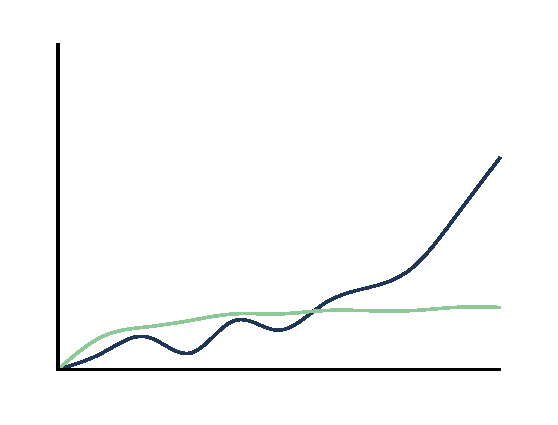
\includegraphics{omega}}%
    \gplfronttext
  \end{picture}%
\endgroup

        \caption{$T(n){\in}\Omega(f(n))$}
    \end{figure}
    \vspace{\stretch{1}}
\end{slide}


\begin{slide}{$\Theta$}
    \vspace{\stretch{1}}
    \begin{defn}
        \myemph{Limite assintótico estrito} $T(n)$ é $\Theta(f(n))$ \textit{se} $T(n)$ é tanto $O(f(n))$ quanto $\Omega(f(n))$.\pause
    \end{defn}
    Dizemos neste caso que $T(n)$ é limitada estritamente por $f(n)$.\pause

    \begin{itemize}
        \item Também conhecido por limite restrito.
        \item A função $T(n)$ cresce dentro de um fator constante multiplicado por $f(n)$.
    \end{itemize}
    \vspace{\stretch{1}}
\end{slide}


\begin{slide}{$\Theta$}
    \vspace{\stretch{1}}
    \begin{figure}
        % GNUPLOT: LaTeX picture with Postscript
\begingroup
  \makeatletter
  \providecommand\color[2][]{%
    \GenericError{(gnuplot) \space\space\space\@spaces}{%
      Package color not loaded in conjunction with
      terminal option `colourtext'%
    }{See the gnuplot documentation for explanation.%
    }{Either use 'blacktext' in gnuplot or load the package
      color.sty in LaTeX.}%
    \renewcommand\color[2][]{}%
  }%
  \providecommand\includegraphics[2][]{%
    \GenericError{(gnuplot) \space\space\space\@spaces}{%
      Package graphicx or graphics not loaded%
    }{See the gnuplot documentation for explanation.%
    }{The gnuplot epslatex terminal needs graphicx.sty or graphics.sty.}%
    \renewcommand\includegraphics[2][]{}%
  }%
  \providecommand\rotatebox[2]{#2}%
  \@ifundefined{ifGPcolor}{%
    \newif\ifGPcolor
    \GPcolortrue
  }{}%
  \@ifundefined{ifGPblacktext}{%
    \newif\ifGPblacktext
    \GPblacktextfalse
  }{}%
  % define a \g@addto@macro without @ in the name:
  \let\gplgaddtomacro\g@addto@macro
  % define empty templates for all commands taking text:
  \gdef\gplbacktext{}%
  \gdef\gplfronttext{}%
  \makeatother
  \ifGPblacktext
    % no textcolor at all
    \def\colorrgb#1{}%
    \def\colorgray#1{}%
  \else
    % gray or color?
    \ifGPcolor
      \def\colorrgb#1{\color[rgb]{#1}}%
      \def\colorgray#1{\color[gray]{#1}}%
      \expandafter\def\csname LTw\endcsname{\color{white}}%
      \expandafter\def\csname LTb\endcsname{\color{black}}%
      \expandafter\def\csname LTa\endcsname{\color{black}}%
      \expandafter\def\csname LT0\endcsname{\color[rgb]{1,0,0}}%
      \expandafter\def\csname LT1\endcsname{\color[rgb]{0,1,0}}%
      \expandafter\def\csname LT2\endcsname{\color[rgb]{0,0,1}}%
      \expandafter\def\csname LT3\endcsname{\color[rgb]{1,0,1}}%
      \expandafter\def\csname LT4\endcsname{\color[rgb]{0,1,1}}%
      \expandafter\def\csname LT5\endcsname{\color[rgb]{1,1,0}}%
      \expandafter\def\csname LT6\endcsname{\color[rgb]{0,0,0}}%
      \expandafter\def\csname LT7\endcsname{\color[rgb]{1,0.3,0}}%
      \expandafter\def\csname LT8\endcsname{\color[rgb]{0.5,0.5,0.5}}%
    \else
      % gray
      \def\colorrgb#1{\color{black}}%
      \def\colorgray#1{\color[gray]{#1}}%
      \expandafter\def\csname LTw\endcsname{\color{white}}%
      \expandafter\def\csname LTb\endcsname{\color{black}}%
      \expandafter\def\csname LTa\endcsname{\color{black}}%
      \expandafter\def\csname LT0\endcsname{\color{black}}%
      \expandafter\def\csname LT1\endcsname{\color{black}}%
      \expandafter\def\csname LT2\endcsname{\color{black}}%
      \expandafter\def\csname LT3\endcsname{\color{black}}%
      \expandafter\def\csname LT4\endcsname{\color{black}}%
      \expandafter\def\csname LT5\endcsname{\color{black}}%
      \expandafter\def\csname LT6\endcsname{\color{black}}%
      \expandafter\def\csname LT7\endcsname{\color{black}}%
      \expandafter\def\csname LT8\endcsname{\color{black}}%
    \fi
  \fi
    \setlength{\unitlength}{0.0500bp}%
    \ifx\gptboxheight\undefined%
      \newlength{\gptboxheight}%
      \newlength{\gptboxwidth}%
      \newsavebox{\gptboxtext}%
    \fi%
    \setlength{\fboxrule}{0.5pt}%
    \setlength{\fboxsep}{1pt}%
\begin{picture}(5040.00,3772.00)%
    \gplgaddtomacro\gplbacktext{%
      \colorrgb{0.12,0.21,0.34}%
      \put(3369,1627){\makebox(0,0)[l]{\strut{}$T(n)$}}%
      \colorrgb{0.90,0.29,0.27}%
      \put(2732,3194){\makebox(0,0)[l]{\strut{}$c1.f(n)$}}%
      \colorrgb{0.55,0.79,0.59}%
      \put(3369,687){\makebox(0,0)[l]{\strut{}$c2.f(n)$}}%
    }%
    \gplgaddtomacro\gplfronttext{%
      \csname LTb\endcsname%
      \put(176,1940){\rotatebox{-270}{\makebox(0,0){\strut{}$tempo$}}}%
      \put(2519,154){\makebox(0,0){\strut{}$n$}}%
    }%
    \gplbacktext
    \put(0,0){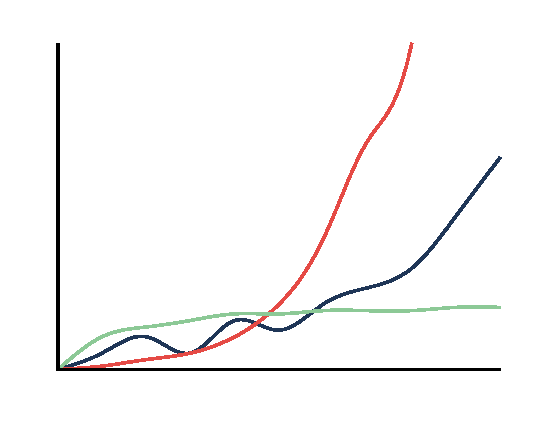
\includegraphics{tight}}%
    \gplfronttext
  \end{picture}%
\endgroup

        \caption{$T(n){\in}\Theta(f(n))$}
    \end{figure}
    \vspace{\stretch{1}}
\end{slide}

\begin{slide}{Observações}
    \vspace{\stretch{1}}
    \begin{itemize}
        \item Dadas duas funções $g=n^2$ e $f=n + 32$, anotamos que $f(n){\in}\mathcal{O}(g(n))$ usando a seguinte notação: $f(n) = \mathcal{O}(g(n))$. 
        \item Neste caso, lemos $f(n)$ \myemph{é} $\mathcal{O}(g(n))$ ao invés de nos referirmos ao sentido de igualdade usual.
        \item Isto porque $\mathcal{O}(g(n))$ é um conjunto de funções que tem o mesmo limite assintótico superior que $g(n)$.
        \item Portanto $f(n)$ é uma função que pertence a esse conjunto.
    \end{itemize}
    \vspace{\stretch{1}}
\end{slide}

%\section{Leituras}

\begin{slide}{Bibliografia consultada}
    \vspace{\stretch{1}}
    \bibliographystyle{acm}
    \bibliography{refs}
    \bibentry{cormen12}
    \bibentry{kleinberg05}
    \vspace{\stretch{1}}
\end{slide}
\end{document}


